\chapter{Pilotforsøg}\vspace{-.75cm}
\textit{Dette bilag beskriver pilotforsøget, som er nødvendigt i forhold til testmåling og design af aktivitetsmåleren. Der undersøges tre forskellige placeringer af sensoren i tre forskellige aktivitetsformer på fire forsøgspersoner.}

\section{Teori}
\textbf{Grundlæggende teori eller henvis tilbage bevægelsesanalysen (Hvis der er en)}

\section{Formål}
For at kunne modificere og tilpasse softwaren til CY8CKIT-043 PSoC 4 M-Series Prototyping Kit er det nødvendigt at kende signalets frekvensindhold og vide, hvordan forskellige aktivitetsformer påvirker sensoren. Målingerne skal undersøges for at kunne lave en algoritme, som kan få sensoren til at skelne imellem de pågældende aktivitetsformer. Derudover skal det bestemmes, hvor sensoren skal placeres på kroppen for mest optimalt udbytte. Derfor er formålet med pilotforsøget følgende:
\begin{itemize}
	\item Bestemme hvordan sensoren påvirkes af gang, løb og cykling.
	\item Undersøge hvor mange g-kræfter sensorens målinger ændrer sig alt efter placering på kroppen.
	\item Bestemme frekvensindholdet for signalet.
\end{itemize}

\section{Materiale}
\begin{itemize}
	\item Løbebånd med justerbar hastighed og sikkerhedssele.
	\item Motionscykel.
	\item Shimmer3 sensor.
	\item Computer med programmet Multi Shimmer Sync version ?.
\end{itemize}

\section{Fremgangsmåde}
Inden forsøget skal computeren med programmet Multi Shimmer Sync forbindes via Bluetooth med Shimmer3 sensoren. Herefter kalibreres Shimmer3 accelerometeret ved hjælp af kalibreringsklodsen og samplingsfrekvensen indstilles til ? Hz. %Alle andre har indstillet til 1024 Hz, men kan ikke sige hvorfor.
Der oprettes en mappe for hver forsøgsperson, som yderligere inddeles i tre mapper efter aktivitetsform. Herunder navngives datafilerne fra målingerne i forhold til placering af sensor, som for eksempel "Forsoegsperson\_1 $\rightarrow$ Gang $\rightarrow$ Ankel".\fxnote{Diskuterres om det er for dybdegående - nogle er for og andre er imod}
Der foretages en testmåling med sensoren, hvor den tændes kortvarigt mens den påvirkes med 1 g. Hvis data fra denne testmåling optages og skildres korrekt er sensoren klar til forsøget.

Forsøget udføres med fire forsøgspersoner. Hver forsøgsperson skal henholdsvis gå, løbe og cykle med sensoren placeret på tre forskellige steder for hver aktivitet. Derudover foretages en måling, hvor forsøgspersonen fra hvile skal nå op til maksspurt med konstant stigningsintervaller. Dette giver $4 x 3 = 12$ målinger for hver forsøgsperson og derfor 48 målinger i alt. Derfor er placering og navngivning af datafilerne yderst essentiel. \\ 
Gang defineres som 3 mph = 4.8 $\sfrac{km}{t}$, løb er 7mph = 11.3 $\sfrac{km}{t}$ og cykling er 13mph = 20.9 $\sfrac{km}{t}$\fxnote{Miles per hour omregnes til kilometer i timen ved at gange med 1.61} \citep{Miles2007}. Inden optagelse af data påbegyndes skal forsøgspersonen have udført den pågældende aktivitet i et minut for at sikre homogen cyklus i den fysiske udførsel. \\
Sensoren skal placeres tre forskellige steder under forsøget på forsøgspersonens højre ben: proximalt over den laterale malleolus, medialt på den ventrale side af tibia og distalt for patella, som illustreret på \figref{fig:sensor_placering}.
\begin{figure}[H]
	\centering
	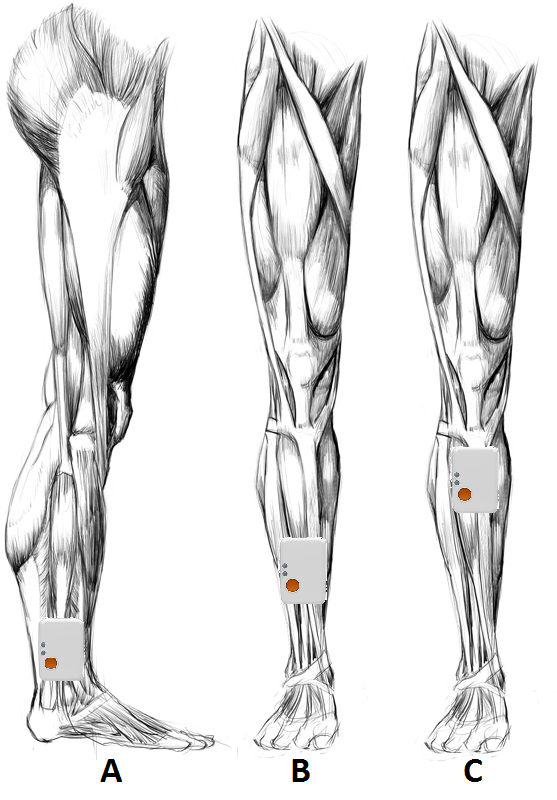
\includegraphics[scale=0.6]{figures/qBilag/Sensor_placering.png}
	\caption{På figuren ses, hvor sensoren skal placeres under pilotforsøget. Placering A viser sensoren siddende proximalt over den laterale malleolus. Placering B illustrerer sensoren, når den er medialt på den ventrale side af tibia. I placering C er sensoren distalt for patella. (Modificeret fra \cite{Perna2016,Shimmer2016})}
	\label{fig:sensor_placering}
\end{figure}
\begin{itemize}
	\item Den første forsøgsperson får fastgjort sensoren i placering A, B eller C - se \figref{fig:sensor_placering} og gør klar til den pågældende aktivitet. Ved aktiviteter på løbebånd skal forsøgspersonen bære sikkerhedssele, som beskytter i tilfælde af fald.
	\begin{itemize}
		\item Ved gang eller løb indstilles løbebåndet til 4.8 eller 11.3 $\sfrac{km}{t}$.
		\item Ved cykling skal forsøgspersonen komme op på 20.9 $\sfrac{km}{t}$.
	\end{itemize}
	\item Den pågældende aktivitet holdes i et minut før målingen påbegyndes. Der optages i 30 sekunder for hver måling.
	\item Efter hver måling skal forsøgspersonen restituere i 10 minutter for at sikre, at der ikke sker en kompensering i gang- eller løbecyklus på grund af træthed. Der tages dog ikke højde for muskeltræthed, da det vurderes, at fysisk aktivitet af denne form ikke vil lede til muskeltræthed inden for disse korte intervaller.\fxnote{Skal vi have en kilde på det her?}
	\item Den fysiske aktivitet gentages tre gange for hver forsøgsperson, da sensoren skal placeres anderledes for hver gang. Sensoren Shimmer3 skal kalibreres for hvert placeringsskifte.
\end{itemize}

\section{Databehandling}

\section{Resultater}

\section{Diskussion}

\section{Konklusion}

%% Opgaver - rettelser
% Man skal markere på forsøgspersonen med tush eller andet hvor sensoren skal placeres
% Skrive ind, at vi også gerne vil se bevægelsesmønsteret på de forskellige ting. Trække sensoren op over knæet
% Gyroskop trækker for meget, fordi skal frekvensen være på 500 Hz